\documentclass[oneside,12pt]{discsthesis}
	\usepackage{graphicx}
	\usepackage{multirow}
	\usepackage{fancyvrb}
	% \usepackage{rotating}
	\usepackage{longtable}
	\usepackage{pdflscape}
	\usepackage{enumerate}
	\usepackage{enumitem}	\setlist[itemize]{leftmargin=*,itemsep=5pt}
	% \usepackage{setspace}
	\usepackage{algpseudocode}
	\usepackage{amsmath}
	\usepackage{amsthm}
	\usepackage[normalem]{ulem}
	\usepackage[titletoc]{appendix}

	\usepackage{algpseudocode}
		\renewcommand{\algorithmiccomment}[1]{\hskip0em$\triangleright$ \emph{#1}}
		\renewcommand{\algorithmicrequire}{\hspace*{6pt}\textbf{Input:}}
		\renewcommand{\algorithmicensure}{\hspace*{6pt}\textbf{Output:}}

	\theoremstyle{plain}
	\newtheorem{thm}{Theorem}

	% \usepackage[justification=centering]{caption}
	% \usepackage[titletoc]{appendix}
	% \graphicspath{ {./contents/img/} }

\begin{document}

	% ------------ Header ------------
	\ThesisAuthor{Mark Joseph D. Ronquillo}
	\ThesisTitle{EMS-GT2: AN IMPROVED EXACT SOLUTION FOR THE (l, d)-PLANTED MOTIF SEARCH PROBLEM}
	\ThesisArea{Computer Science}
	\ThesisDefenseYear{2016}
	\DefenseDate{October 24, 2016}
	% \ThesisGrade{}

	\DepartmentHead{MARLENE M. DE LEON, Ph.D.}
	\SchoolHead{EVANGELINE P. BAUTISTA, Ph.D.}
	\ThesisAdviser{PROCESO L. FERNANDEZ, JR., Ph.D.}

	\FirstPanelMember{ANDREI D. CORONEL, Ph.D.}
	\SecondPanelMember{JULIETA Q. NABOS, Ph.D.}
	\ThirdPanelMember{JOSE ALFREDO A. DE VERA III}

	\ThesisStyle{MS}{FinalWithCorner}{-10pt}{15pt}

	% ------------ Paper's Content ------------ 
	\FrontMatter
		% \input{frontmatter/acknowledgements}
		\begin{acknowledgments}

	First, I would like to thank my God and my Savior Jesus Christ for all the blessings He has given to me and all the lessons He has taught me. I also extend my deepest gratitude to my adviser Dr. Proceso Fernandez for teachings and the knowledge that he has imparted to me. To the Computer Algorithms and Analysis lab people and my peers, thank you for all the support. Lastly, I also would like to thank my panelists Dr. Andrei Coronel, Dr. Julieta Nabos and Mr. Alfredo De Vera. 

	This work is funded and supported by the DOST's Engineering Research and Development for Technology (ERDT).

	Thank you and let's all aim for excellence in our lives. May God bless us all.
	
\end{acknowledgments}

		
\begin{abstract}\boldmath Finding DNA motifs is a widely studied area in the field of Computational Biology. Motifs signify different information that are useful for biologists like discovering transcription factor-binding sites and helps them identify potential therapeutic drug target. There are several variations of the motif finding problem, and one of these is called the (l,d)-motif search or Planted Motif Search problem (PMS). In this paper, we propose the EMS-GT2 algorithm, an extension of the Exact Motif Search - Generate and Test (EMS-GT) which is an exact enumerative algorithm for PMS. In EMS-GT2, we incorporated a new speedup technique that is based on an important property that we have discovered, which we prove in this paper, and which has enabled a more efficient block-processing of candidate motifs. Our C++ implementation of EMS-GT2 running on synthetic data for several PMS challenge instances demonstrate that it is competitive with both the EMS-GT and qPMS9, the two current best exact solutions for PMS. In particular, EMS-GT2 is able to reduce the run-times of EMS-GT by 20.3\%, 15.8\% and 22.6\% for the (l,d) challenge instances (13, 4), (15, 5) and (17, 6) respectively. It also outperforms qPMS9, having runtime reductions of 91.6\%, 79.3\%, 82.0\%, 59.4\% and 9.7\% for the (9, 2), (11, 3), (13, 4), (15, 5) and (17, 6) synthetic challenge instances respectively.

	
\end{abstract}

		\tableofcontents
		\listoffigures
		\listoftables

	\MainMatter
		% CHAPTER 1
		\chapter{INTRODUCTION}
			
% A bit of introduction on significance
DNA motif finding is a well studied topic in computational biology. Motif is a short patterns of interests that occurs in large amount of biological data. Detection of these motifs often leads to new biological discoveries. These may lead to finding transcription factor-binding sites that helps biologists understand gene functions. Additionally, it helps understand human diseases, identify potential therapeutic drug target and conclude commonalities from different species.

% Definition of PMS
There are many variations of the motif search problem such as Simple Motif Search (SMS), Edit-distance-based Motif Search (EMS) and Planted Motif Search (PMS) also known as $(l, d)$-motif search. This study focuses on the exact enumerative algorithm for the PMS problem. Planted Motif Search is formally defined in \cite{ExactAlgorithmsPMS} as \emph{Input are $t$ sequences of length $n$ each. Input also are two integers $l$ and $d$. The problem is to find a motif (i.e., a sequence) $M$ of length $l$. It is given that each input sequence contains a variant of $M$ . The variants of interest are sequences that are at a hamming distance of $d$ from $M$}. In solving the PMS problem, traditional string matching won't be efficient since these biological motifs are not typically exact but are subject to mutations. As a matter of fact, PMS has already been proven to be NP-complete, which means that it is very unlikely to have an algorithm that solves it in polynomial time \cite{Evans2003407}.

In this study we introduce EMS-GT2 an improved version of the EMS-GT algorithm that implements a series of speedup techniques that use the block processing, introduced in \cite{sia2015}, in different areas of the algorithm. EMS-GT2 also improves the way it computes the hamming distance by pre-computing the non-zero pairs of bits for every integer of a given number of bits.

				\section{Context of the Study}

This section formally defines the $(l, d)$-planted motif search problem and some related terms that are commonly used in this study. \newline

% l-mer
\noindent{\bf\boldmath DEFINITION 1. $l$-mer} \newline
\noindent An \textbf{\boldmath $l$-mer} is a string of length $l$ in the alphabet $\Sigma$. In this study, $\Sigma$ = \{\texttt{a}, \texttt{c}, \texttt{g}, \texttt{t}\} since we are dealing with DNA sequences. Formally, an $l$-mer is an element of the set $\Sigma^l$. 

\noindent \hspace*{35pt} Ex. \texttt{agagt} is a $5$-mer and \texttt{agagtca} is a $7$-mer.  \newline

% Hamming distance
\noindent{\bf\boldmath DEFINITION 2. Hamming distance $d_H$} \newline
\noindent The \textbf{\boldmath Hamming distance $d_H$} between two $l$-mers, of equal length, is equal to the number of positions where the $l$-mers have mismatches. 

\noindent \hspace*{35pt} Ex. $d_H(\texttt{\uline{a}ct\uline{tg}ca}, \texttt{\uline{t}ct\uline{aa}ca}) = 3$.\newline
\noindent \hspace*{55pt} the underlined characters represents the mismatch positions. \newline

% d-neighbor
\noindent{\bf\boldmath DEFINITION 3. $d$-neighbor} \newline
\noindent An $l$-mer $x$ is considered a \textbf{\boldmath $d$-neighbor} of another $l$-mer $y$ if the Hamming distance between the two is at most $d$.

\noindent \hspace*{35pt} Ex. Given two $7$-mers, $\texttt{\uline{a}tta\uline{g}ct}$ and $\texttt{\uline{g}tta\uline{c}ct}$ are $d$-neighbors, \newline
\noindent \hspace*{55pt} where $d \geq 2$. \newline

% d-neighborhood of an l-mer
\noindent{\bf\boldmath DEFINITION 4. $d$-neighborhood of an $l$-mer $x$} \newline
\noindent The \textbf{\boldmath $d$-neighborhood of an $l$-mer $x$} is the set {\boldmath $N(x, d)$} of all $l$-mers with at most $d$ Hamming distance from $x$. i.e., {\boldmath $d_H (x, x') \leq d$}.

\noindent \hspace*{35pt} Ex. \texttt{ccgga}, \texttt{ccaaa}, and \texttt{gctta} are all in $N(\texttt{cctta}, 2)$ where $l = 5$. \newline

% d-neighborhood of a sequence
\noindent{\bf\boldmath DEFINITION 5. $d$-neighborhood of a sequence $S$} \newline
\noindent The \textbf{\boldmath $d$-neighborhood of a sequence $S$} is the set {\boldmath $\mathcal{N}(S, d)$} of all $d$-neighbors of all $l$-mers in sequence $S$. 
	
\noindent \hspace*{35pt} Ex. {\small $\mathcal{N}(\texttt{aattacg}, 2) = N(\texttt{aatta}, 2) \cup N(\texttt{attac}, 2) \cup N(\texttt{ttacg}, 2)$} \newline
\noindent \hspace*{55pt} where $l = 5$. \newline

\noindent{\bf\boldmath DEFINITION 6. $(l, d)$ Planted Motif Problem} \newline
\noindent Given a set of $n$ sequences, where each sequence is of length $m$, an $l$ and $d$ integer values, the goal is to find a motif of length $l$. It is also given that a $d$-neighbor of the motif is planted in each of the $n$ sequence exactly once at a random position.

				\section{Objectives of the study}

This study aims to improve the runtime performance of the EMS-GT algorithm and propose a new version of the algorithm, referred to as the EMS-GT2 algorithm. The objectives of the study are as follows:

\begin{enumerate}
	\item To explore additional speedup techniques that may be used to improve the runtime performance of the EMS-GT algorithm.

	\item To evaluate the runtime performance of the proposed EMS-GT2 algorithm using synthetic datasets.

	\item To compare the performance of the EMS-GT2 against its predecessor EMS-GT and the qPMS9 algorithm using synthetic datasets.
\end{enumerate}
				\section{Research questions}

This study aims to answer the following questions:

\begin{itemize}
	\item How can we further improve the runtime performance of EMS-GT algorithm?

	\item What is the runtime performance of the proposed EMS-GT2 on the synthetic datasets?

	\item What is the performance of the proposed EMS-GT2 compared to its predecessor EMS-GT and to qPMS9 algorithm?	
\end{itemize}
				\section{Significance of the study}
% Rephrase
Motif signifies important information that is use the field of Computational Biology. Finding these motifs, which is already proven as NP-Complete problem, requires creative, fast and efficient algorithms. Improving an already established and competitive algorithm in the motif finding is one way to contribute to this field.

Motif usually signifies important information that are useful in the field of Computational Biology. 


EMS-GT algorithm is competitive and able to beat current state-of-the-art algorithms like PMS8 and qPMS9 in a certain range of problem instances. Improving EMS-GT in such a way that it can beat other algorithms in different problem instances will make it more viable option in practical motif finding applications. In addition, the improved way of hamming distance computation and the discovered properties of the data structure that EMS-GT2 use may proved useful in other algorithm solutions that use such data structure.

				\section{Scope and limitations}

This study focuses on improving the existing EMS-GT by exploring and optimizing different areas in the algorithm and thus proposing the EMS-GT2 algorithm. Since EMS-GT2 introduces a memory contstraint when $l$ is sufficiently large, each new speedup technique was evaluated using all synthetic datasets of ($l$, $d$)-challenge instance where $l < 18$. Finally, EMS-GT2 doesn't have the capability to run on multiple processors and, thus, we evaluate the algorithms in a single-processor execution.

		% CHAPTER 2
		\chapter{REVIEW OF RELATED LITERATURE}
			\section{Review of Related Literature}
	Motif finding has been studied extensively in the previous years. Numerous algorithms have been made for motif finding and for PMS. These algorithms are categorized as either approximate algorithms or exact algorithms. Approximate algorithms, although it is fast, do not guarantee the exact solution all the time. Heuristic algorithms that perform local search such as Gibbs Sampling, Expectation Maximization (EM),  Projections etc. are previously explored in the literature. Most of these algorithms initially work on a tuple of alignment positions that corresponds to $l$-mers across different string sequences in the dataset. Then iteratively refine the alignment until a certain criteria has met. MEME \cite{Bailey2006} is a tool for motif finding that implements Expected Maximization. Other approximate algorithms that use local search are GARP \cite{huo2009combining}, GibbsDNA \cite{lawrence1993detecting} and Random Projection \cite{Buhler2001Tompa, huo2009combining}. WINNOWER \cite{pevzner2000combinatorial} reduces the PMS problem into finding a large clique in a multipartite graph. Instead of looking for the motif directly, the algorithm applies a winnowing technique to remove spurious edges that trims the graph representation making it easier to find the motif. Other approximate algorithms are MULTIPROFILER \cite{Keich01102002},  PatternBranching, ProfileBranching \cite{Price27092003} and CONSENSUS \cite{hertz1999identifying};

	% explain one or two approximate then list the rest

	Although it is not as fast as approximate algorithms, exact algorithms return the correct answer all the time. Furthermore, these exact algorithms can be categorized based on their approach in solving the problem. One approach is to generate a common neighborhood out of all $(m - l + 1)^n$ possible positions or $l$-mers from all string sequences. This approach is called sample-driven. Another approach is called pattern-driven that checks from $\Sigma^l$ possible $l$-mers which are the motifs. 

	% PMS Series
	Rajasekaran et. al. proposed a series of exact algorithms for the $(l, d)$-motif search problem. The algorithm PMS1 \cite{ExactAlgorithmsPMS} is one of these algorithms. PMS1 solves the problem by enumerating the $d$-neighborhood of all the sequences in the dataset and intersects them, the result is the set of motifs. PMSi and PMSP \cite{Davila2006} are algorithms based on PMS1. PMSi improves the memory space requirement of PMS1 by processing only two sequences at a time. PMSP works by generating all the $d$-neighborhood of each $l$-mer in the first sequence and testing each $d$-neighbor if it exists in the remaining sequences. PMSPrune \cite{pms2007} works the same as PMP but with some improvements. It generates the neighborhood of an $l$-mer using a branch and bound approach and implements a pruning strategy to speedup the testing of $l$-mers. Succeeding algorithms like PMS5 \cite{Dinh2011} and PMS6 \cite{Shibdas2014} extend the ideas of PMS1 and PMSPrune. PMS5 generates the common neighborhood of three $l$-mers from different sequences at a time and uses ILP for the pruning process. PMS6 only differs from PMS5 in the way it determines the three $l$-mers. Quorum PMS is a generalized version of the $(l, d)$-motif search problem. Instead of finding an $l$-mer that exists in all $n$ sequences, it only considers up to $q$. We can see that a qPMS problem is equal to PMS when $q = n$. The qPMS7 \cite{Dinh2012} is one algorithm that solves the qPMS problem. Algorithm qPMS7 is a generalized version of qPMSPrune (quorum version of PMSPrune) combined with the pruning strategy of PMS5 algorithm. PMS8 \cite{pms2014} is an algorithm that combines the sample-driven approach and the pattern-driven approach. First, it chooses $k$-tuple $T$ of $l$-mers from $k$ different sequences and it makes sure that all $l$-mers in $T$ has a common neighbor. Each $l$-mer that belongs to the common neighborhood of the tuple $T$ will be checked if it appears in the remaining $n - k$ sequences. The current state-of-the-art algorithm qPMS9 \cite{pms2015} improves the sample-driven approach of PMS8 by prioritizing $l$-mers that are highly distant from those already in the tuple resulting in a smaller size of common $d$-neighborhood to test and enables the algorithm to process the quorum version of the PMS problem.

	% Bitbased and Voting 
	Many exact algorithms solve the PMS problem using suffix trees and other related data structures. RISO \cite{Carvalho05ahighly}, RISOTTO \cite{Pisanti06risotto}, SPELLER \cite{Sagot98spellingapproximate} and SMILE are all exact algorithms that use suffix trees. MITRA \cite{eskin2002finding} improves the excessive memory requirement of sample-driven approach by using mismatch tree. Two other algorithms that are similar in how our algorithm works are the Voting algorithm and Bit-based algorithm. Voting algorithm \cite{Chin2005} maintains a hash table that tracks the number the occurrence of every possible $l$-mer and makes sure that every $l$-mer is only counted once in each sequence. An $l$-mer is considered a motif if its total occurrences is equal to the total number of sequences in the dataset. Bit-based algorithm \cite{dasari2010efficient} generates the neighborhood of each sequence and intersects it to get the set of motif. Unlike PMS1, the Bit-based algorithm maps every $l$-mer to its corresponding integer value. It uses an array of size $\Sigma^l$ to represent the neighborhood of a sequence and uses the integer representation of an $l$-mer to flag if its a member of the array. It generates the neighborhood of all sequences and merges it using the logical operator AND. The resulting array represents the set of motif.

			% 
The Exact Motif Search - Generate and Test algorithm for the planted motif search problem, first developed by Nabos \cite{nabos2015dissertation}, is composed of main two phases, the Generate phase and the Test phase. The Generate phase takes the first $n'$ number of string sequences in the dataset and generates the set $d$-neighborhood one sequence at a time then intersects it. This accumulates and outputs the set of candidate motifs $\mathcal{C}$ and is composed of $l$-mers that have at least one $d$-neighbor in each of the first $n'$ sequences. The Test phase evaluates each candidate motif $c \in C$ by comparing $c$ if it has at least one $d$-neighbor in each of the remaining $n - n'$ string sequences. \newline

\noindent These phases are formally defined below:
% show the formal definition of EMS-GT algorithm steps
\begin{enumerate} [label={\em (\alph*)}]

	\item {Generate phase} \newline
	This phase operates on the first $n'$ sequences. The intersection of the $d$-neighborhood of each sequence will result to the set of candidate motifs $C$.\newline

	\begin{equation}
		C = \mathcal{N}(S_{1}, d) \cap \mathcal{N}(S_{2}, d) \cap...\cap \mathcal{N}(S_{n'}, d).
	\end{equation} 

	\item {Test phase}\newline
	Each candidate motif in $C$ will be evaluated if it appears in all of the remaining $n - n'$ string sequences. If a candidate motif pass the test, it is then included in the set of motifs $M$. 

\end{enumerate}

% 
The Exact Motif Search - Generate and Test algorithm for the planted motif search problem, first developed by Nabos \cite{nabos2015dissertation}, is composed of main two phases, the Generate phase and the Test phase. The Generate phase takes the first $n'$ number of string sequences in the dataset and generates the set $d$-neighborhood one sequence at a time then intersects it. This accumulates and outputs the set of candidate motifs $\mathcal{C}$ and is composed of $l$-mers that have at least one $d$-neighbor in each of the first $n'$ sequences. The Test phase evaluates each candidate motif $c \in C$ by comparing $c$ if it has at least one $d$-neighbor in each of the remaining $n - n'$ string sequences. \newline

\noindent These phases are formally defined below:
% show the formal definition of EMS-GT algorithm steps
\begin{enumerate} [label={\em (\alph*)}]

	\item {Generate phase} \newline
	This phase operates on the first $n'$ sequences. The intersection of the $d$-neighborhood of each sequence will result to the set of candidate motifs $C$.\newline

	\begin{equation}
		C = \mathcal{N}(S_{1}, d) \cap \mathcal{N}(S_{2}, d) \cap...\cap \mathcal{N}(S_{n'}, d).
	\end{equation} 

	\item {Test phase}\newline
	Each candidate motif in $C$ will be evaluated if it appears in all of the remaining $n - n'$ string sequences. If a candidate motif pass the test, it is then included in the set of motifs $M$. 

\end{enumerate}

% 
The Exact Motif Search - Generate and Test algorithm for the planted motif search problem, first developed by Nabos \cite{nabos2015dissertation}, is composed of main two phases, the Generate phase and the Test phase. The Generate phase takes the first $n'$ number of string sequences in the dataset and generates the set $d$-neighborhood one sequence at a time then intersects it. This accumulates and outputs the set of candidate motifs $\mathcal{C}$ and is composed of $l$-mers that have at least one $d$-neighbor in each of the first $n'$ sequences. The Test phase evaluates each candidate motif $c \in C$ by comparing $c$ if it has at least one $d$-neighbor in each of the remaining $n - n'$ string sequences. \newline

\noindent These phases are formally defined below:
% show the formal definition of EMS-GT algorithm steps
\begin{enumerate} [label={\em (\alph*)}]

	\item {Generate phase} \newline
	This phase operates on the first $n'$ sequences. The intersection of the $d$-neighborhood of each sequence will result to the set of candidate motifs $C$.\newline

	\begin{equation}
		C = \mathcal{N}(S_{1}, d) \cap \mathcal{N}(S_{2}, d) \cap...\cap \mathcal{N}(S_{n'}, d).
	\end{equation} 

	\item {Test phase}\newline
	Each candidate motif in $C$ will be evaluated if it appears in all of the remaining $n - n'$ string sequences. If a candidate motif pass the test, it is then included in the set of motifs $M$. 

\end{enumerate}

% \input{contents/pseudocode/ems-gt}

% \input{contents/pseudocode/recursive-neighborhood-gen}

Data structures and the how an algorithm deals with the data commonly drive the performance of an algorithm. The EMS-GT algorithm uses a compressed bit-flag array for fast candidate motif elimination. Some key techniques that EMS-GT uses are defined in this section.

	\subsubsection{Integer mapping of $l$-mers}
	EMS-GT converts $l$-mers into its corresponding integer values. To achieve this, each character in the $l$-mer is translated using 2 bits (a=00, c=01, g=10, t=11). \newline
		{\small Ex.	\texttt{actg} maps to \texttt{00011110} and has an integer value of 30} 

	\subsubsection{Bit-based set representation and l-mer enumeration} 
	The EMS-GT maintains a $4^l$ array for enumerating all the possible $l$-mer values. The $l$-mer's integer value is used as the index value for the array. It uses the value of 1 if the $l$-mer is a member of the set, else it sets the value to 0.

	\subsubsection{Bit-array compression}
	To efficiently store these $l$-mers and save memory space, EMS-GT implements an approach that compresses the search space array using integer value bit flags. Instead of one $l$-mer per index value, the implementation can flag up to 32 $l$-mers (since we are using 32-bit integers) per index value. The explanation on how the algorithm accesses the bit flag is defined below: \newline

		{\small Ex. \texttt{gacgt} maps to \texttt{1000011011} = 539 in decimal.\newline
			\hspace*{64pt} \emph{bit position} = 539 mod 32 = 27;\newline
			\hspace*{64pt} \emph{array index}  = 539 / 32 = 16;\newline
			\hspace*{64pt} The bit flag for \texttt{gacgt} is in the 27$^{th}$ least significant bit\newline
			\hspace*{64pt} of the integer at array index 16.}

	\input{contents/00_figure/search_space}

	\subsubsection{XOR-based Hamming distance computation}
	The mapping of an $l$-mer to its integer value has an additional advantage in computing for mismatch positions. Applying the boolean operator exclusive-or (XOR) between two integer values will return another integer value that contains nonzero value for mismatch position. Counting this nonzero positions result to the hamming distance value. An example of this computation is shown below: \newline

	{\small Ex.	\texttt{aacgt} maps to \texttt{0000011011} \newline
		\vspace*{2pt}\hspace*{53pt} \underline{\texttt{tacgc} maps to \texttt{1100011001}} \newline
		\hspace*{55pt}	XOR produces \texttt{\uline{11}000000\uline{10}} = 2 mismatches.} \newline
		\hspace*{53pt} (Note, the mismatches are counted per pair)


	\subsubsection{Recursive neighborhood generation}
	The Generate step of the algorithm produces the $d$-neighborhood of a string sequence by generating the $d$-neighborhood of all $l$-mers in that sequence. Our implementation of EMS-GT uses a recursive approach for generating the $d$-neighborhood of an $l$-mer. The recursive generation can be visualized by a tree $\mathcal{T}(x)$ of height $d$ that is generated in depth-first manner. Each node is a tuple of $(w, p)$ where $w$ is an $l$-mer and $p$ corresponds to a position in the $l$-mer $0 \leq p \leq l$. At a given node $(w, p)$ and $p \neq l$, three children nodes are generated where each node is variant of $w$ that has a different character in $p + 1$ position. The root node is $(x, 0)$ and any $l$-mer in nodes at depth $t$ has a hamming distance of $t$ from the $l$-mer $x$. Given this, the expected size of $N(x, d)$ can be computed using the equation: \newline
	\begin{equation}
		|N(x,d)| = \sum_{i=0}^d \binom{l}{i} 3^{i}
	\end{equation}

	\input{contents/00_figure/neighborhood_generation}

	\subsubsection{Block-based optimization for neighborhood generation}
	The way EMS-GT represents the $d$-neighborhood $N_x$ of $l$-mer $x$ opens up a new way to improve the generation of neighborhood. $N_x$ is represented by a compresed $4^l$ bit flags array, where value of 1 corresponds to set membership, 0 if otherwise.  A previous study by Sia \cite{sia2015} improved the runtime performance in generating $N_x$. If $N_x$ is partitioned into blocks of $4^k$ bits each, where $k < l$, each block will conform into ($k$ + 2) bit patterns. By pre-computing these patterns, the algorithm can build the $N_x$ by blocks of bits instead of one bit at a time.

	\input{contents/00_figure/bit-patterns}

	The algorithm divides the $l$-mer $x$ into its $(l - k)$-length prefix $y$ and suffix $z$ of length $k$. With the block patterns of $4^k$ $l$-mers generated, the algorithm recursively generates all possible prefix of $x$. For each prefix $y'$ generated, the algorithm applies the corresponding block pattern in $N_x$ based on $z$ and the remaining number of allowed mutations $d'$, where $d' = d - d_H(y, y')$. Specifically, EMS-GT builds the $\mathcal{N}_S$ using these steps:

	\begin{enumerate}
		\item Initialize $\mathcal{N}_S$ as an array of $4^l$ bits set to zero, and select a value for $k$.

		\item Pre-generate {\em Pattern}( $z$, $d_z$ ) for all $z \in \Sigma^k$ and all $d_z \in \{1,...,k-1\}$ to serve as bit masks for blocks. Note that block patterns for $d_z=0$ (one bit set) and $d_z=k$ (all bits set) will not require bit masks.

		\item For each $l$-mer $x = yz$ in sequence $S$: take each neighbor $y'$ of $y$, find the block in $\mathcal{N}_S$ whose prefix is $y'$, and compute the allowable suffix mismatches $d_z = d - d_H(y,y')$ within this block. Then,

			\begin{enumerate}
				\item if $d_z = 0$, set the bit at position $z$ in the block;
				\item if $d_z \geq k$, set all bits in the block to 1;
				\item otherwise, mask {\em Pattern}( $z$, $d_z$ ) onto the block.
			\end{enumerate}
	\end{enumerate}

	Choosing the optimum value for $k$ is important in this speedup technique. The $k$ value determines the runtime complexity of this technique since $k$ value determines the size of the block patterns. When $k$ value is higher, there are fewer prefix to generate recursively but each block bits setting is large. When $k$ value is lower, block bits setting is small but the algorithm has to recursively generate a larger number of prefix value of $l$-mer $x$. The optimum $k$ value used in the study is 5.

	\input{contents/00_pseudocodes/block-pattern-generation}

	% Elaborate and include results
	% Mention its competitiveness and a bit of introduction on possible areas of improvement 
	EMS-GT with this speedup technique has proven its competitiveness against algorithms qPMSPrune, qPMS7, PMS8 and qPMS9. Previous experimentations showed that EMS-GT with this speedup technique outperforms PMS8 in challenge instances (9, 2), (11, 3), (13, 4), (15, 5) and (17, 6). Compared to qPMS9, the improved EMS-GT is faster on all challenge instances mentioned except (17, 6). This study aims to outperform qPMS9 for challenges up to (17, 6).

	\input{contents/00_figure/sia-bar-results}

% \begin{figure}[b]
	\noindent \hspace*{6pt}{\bf Algorithm 2} \textsc{Generate Neighborhood}
	\begin{algorithmic}[1]
		\label{alg:recursive-nbr-gen}
		\Require DNA sequence $S$, motif length $l$, mismatches $d$
		\Ensure bit-array $\mathcal{N}$ representing $\mathcal{N}(S,d)$ \vspace*{6pt}
		% \For{$i \leftarrow$ 1 to $4^{l}$}
		\State $\mathcal{N}[i] \leftarrow 0,\ \ \forall i < 4^{l}$ 
		% \EndFor
		\For{each $l$-mer $x$ in $S$}
			\State \textsc{AddNeighbors}($x$, 0, $d$) \hspace*{9pt}\Comment{recursive procedure}
		\EndFor
		\State \Comment{make $d$ changes in $l$-mer $x$, from position $s$ onward}
		\Procedure{AddNeighbors}{$x$, $s$, $d$}
			\For{$i \leftarrow s$ to $l$}
				\State $\Sigma \leftarrow$ \{\texttt{a}, \texttt{g}, \texttt{c}, \texttt{t}\} $- x_{i}$ \hspace*{6pt}\Comment{$i^{th}$ character in $x$}
				\For{$j \leftarrow 1$ to $|\Sigma|$}
					\State $neighbor \leftarrow\ ${\em\small concatenate}$(x_{1...i-1},\Sigma_{j},x_{i+1...l})$
					\State $\mathcal{N}[neighbor] \leftarrow 1$
					\If{$d > 1$ and $i < l$}
						\State \textsc{AddNeighbors}($neighbor$, $i+1$, $d-1$)
					\EndIf
				\EndFor
			\EndFor
		\EndProcedure
		\State\Return $\mathcal{N}$
	\end{algorithmic}
\end{figure}

Data structures and the how an algorithm deals with the data commonly drive the performance of an algorithm. The EMS-GT algorithm uses a compressed bit-flag array for fast candidate motif elimination. Some key techniques that EMS-GT uses are defined in this section.

	\subsubsection{Integer mapping of $l$-mers}
	EMS-GT converts $l$-mers into its corresponding integer values. To achieve this, each character in the $l$-mer is translated using 2 bits (a=00, c=01, g=10, t=11). \newline
		{\small Ex.	\texttt{actg} maps to \texttt{00011110} and has an integer value of 30} 

	\subsubsection{Bit-based set representation and l-mer enumeration} 
	The EMS-GT maintains a $4^l$ array for enumerating all the possible $l$-mer values. The $l$-mer's integer value is used as the index value for the array. It uses the value of 1 if the $l$-mer is a member of the set, else it sets the value to 0.

	\subsubsection{Bit-array compression}
	To efficiently store these $l$-mers and save memory space, EMS-GT implements an approach that compresses the search space array using integer value bit flags. Instead of one $l$-mer per index value, the implementation can flag up to 32 $l$-mers (since we are using 32-bit integers) per index value. The explanation on how the algorithm accesses the bit flag is defined below: \newline

		{\small Ex. \texttt{gacgt} maps to \texttt{1000011011} = 539 in decimal.\newline
			\hspace*{64pt} \emph{bit position} = 539 mod 32 = 27;\newline
			\hspace*{64pt} \emph{array index}  = 539 / 32 = 16;\newline
			\hspace*{64pt} The bit flag for \texttt{gacgt} is in the 27$^{th}$ least significant bit\newline
			\hspace*{64pt} of the integer at array index 16.}

	\begin{figure}[h]
	\centering
	\label{fig:search_space}
	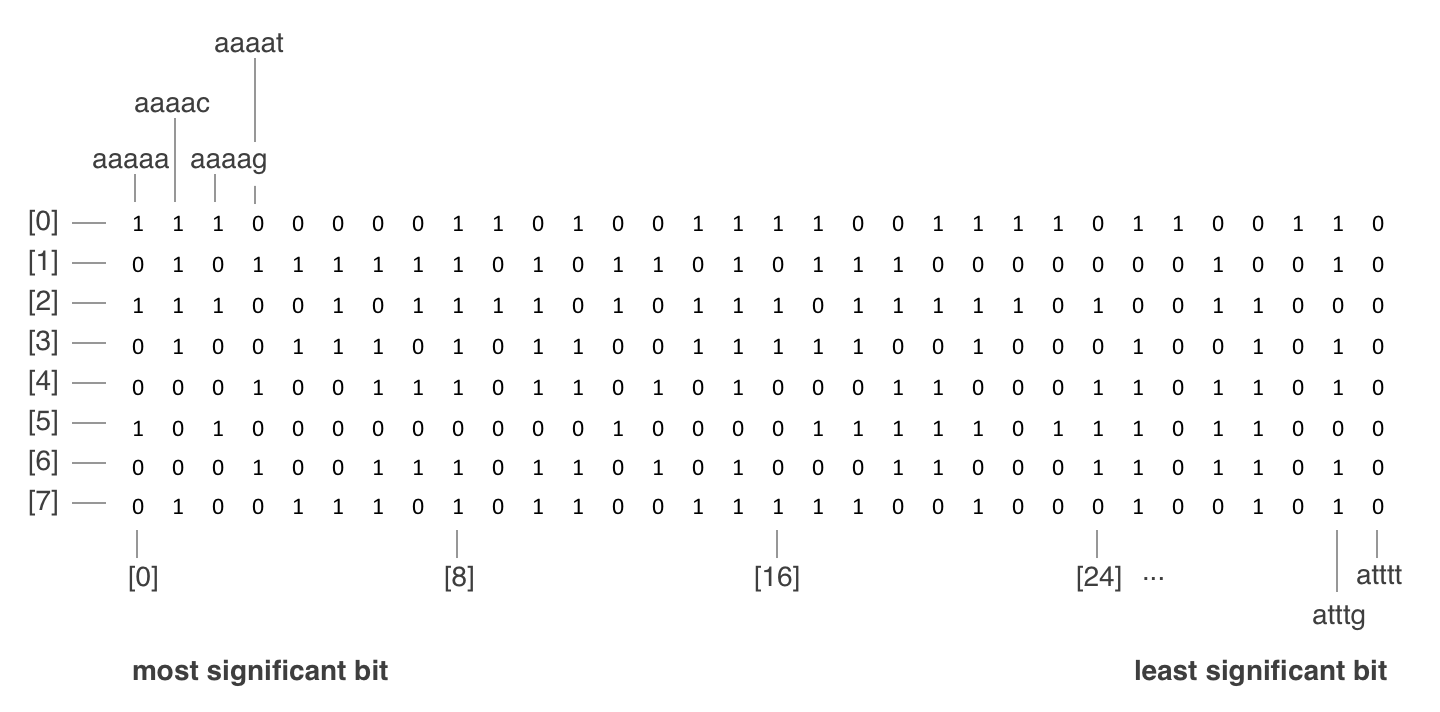
\includegraphics[width=5in]{contents/00_images/search_space}\vspace*{5pt}
	\caption{First 8 rows of the $4^{5}$ search space with random flag values.}
\end{figure}

	\subsubsection{XOR-based Hamming distance computation}
	The mapping of an $l$-mer to its integer value has an additional advantage in computing for mismatch positions. Applying the boolean operator exclusive-or (XOR) between two integer values will return another integer value that contains nonzero value for mismatch position. Counting this nonzero positions result to the hamming distance value. An example of this computation is shown below: \newline

	{\small Ex.	\texttt{aacgt} maps to \texttt{0000011011} \newline
		\vspace*{2pt}\hspace*{53pt} \underline{\texttt{tacgc} maps to \texttt{1100011001}} \newline
		\hspace*{55pt}	XOR produces \texttt{\uline{11}000000\uline{10}} = 2 mismatches.} \newline
		\hspace*{53pt} (Note, the mismatches are counted per pair)


	\subsubsection{Recursive neighborhood generation}
	The Generate step of the algorithm produces the $d$-neighborhood of a string sequence by generating the $d$-neighborhood of all $l$-mers in that sequence. Our implementation of EMS-GT uses a recursive approach for generating the $d$-neighborhood of an $l$-mer. The recursive generation can be visualized by a tree $\mathcal{T}(x)$ of height $d$ that is generated in depth-first manner. Each node is a tuple of $(w, p)$ where $w$ is an $l$-mer and $p$ corresponds to a position in the $l$-mer $0 \leq p \leq l$. At a given node $(w, p)$ and $p \neq l$, three children nodes are generated where each node is variant of $w$ that has a different character in $p + 1$ position. The root node is $(x, 0)$ and any $l$-mer in nodes at depth $t$ has a hamming distance of $t$ from the $l$-mer $x$. Given this, the expected size of $N(x, d)$ can be computed using the equation: \newline
	\begin{equation}
		|N(x,d)| = \sum_{i=0}^d \binom{l}{i} 3^{i}
	\end{equation}

	\begin{figure}[h]
	\centering
	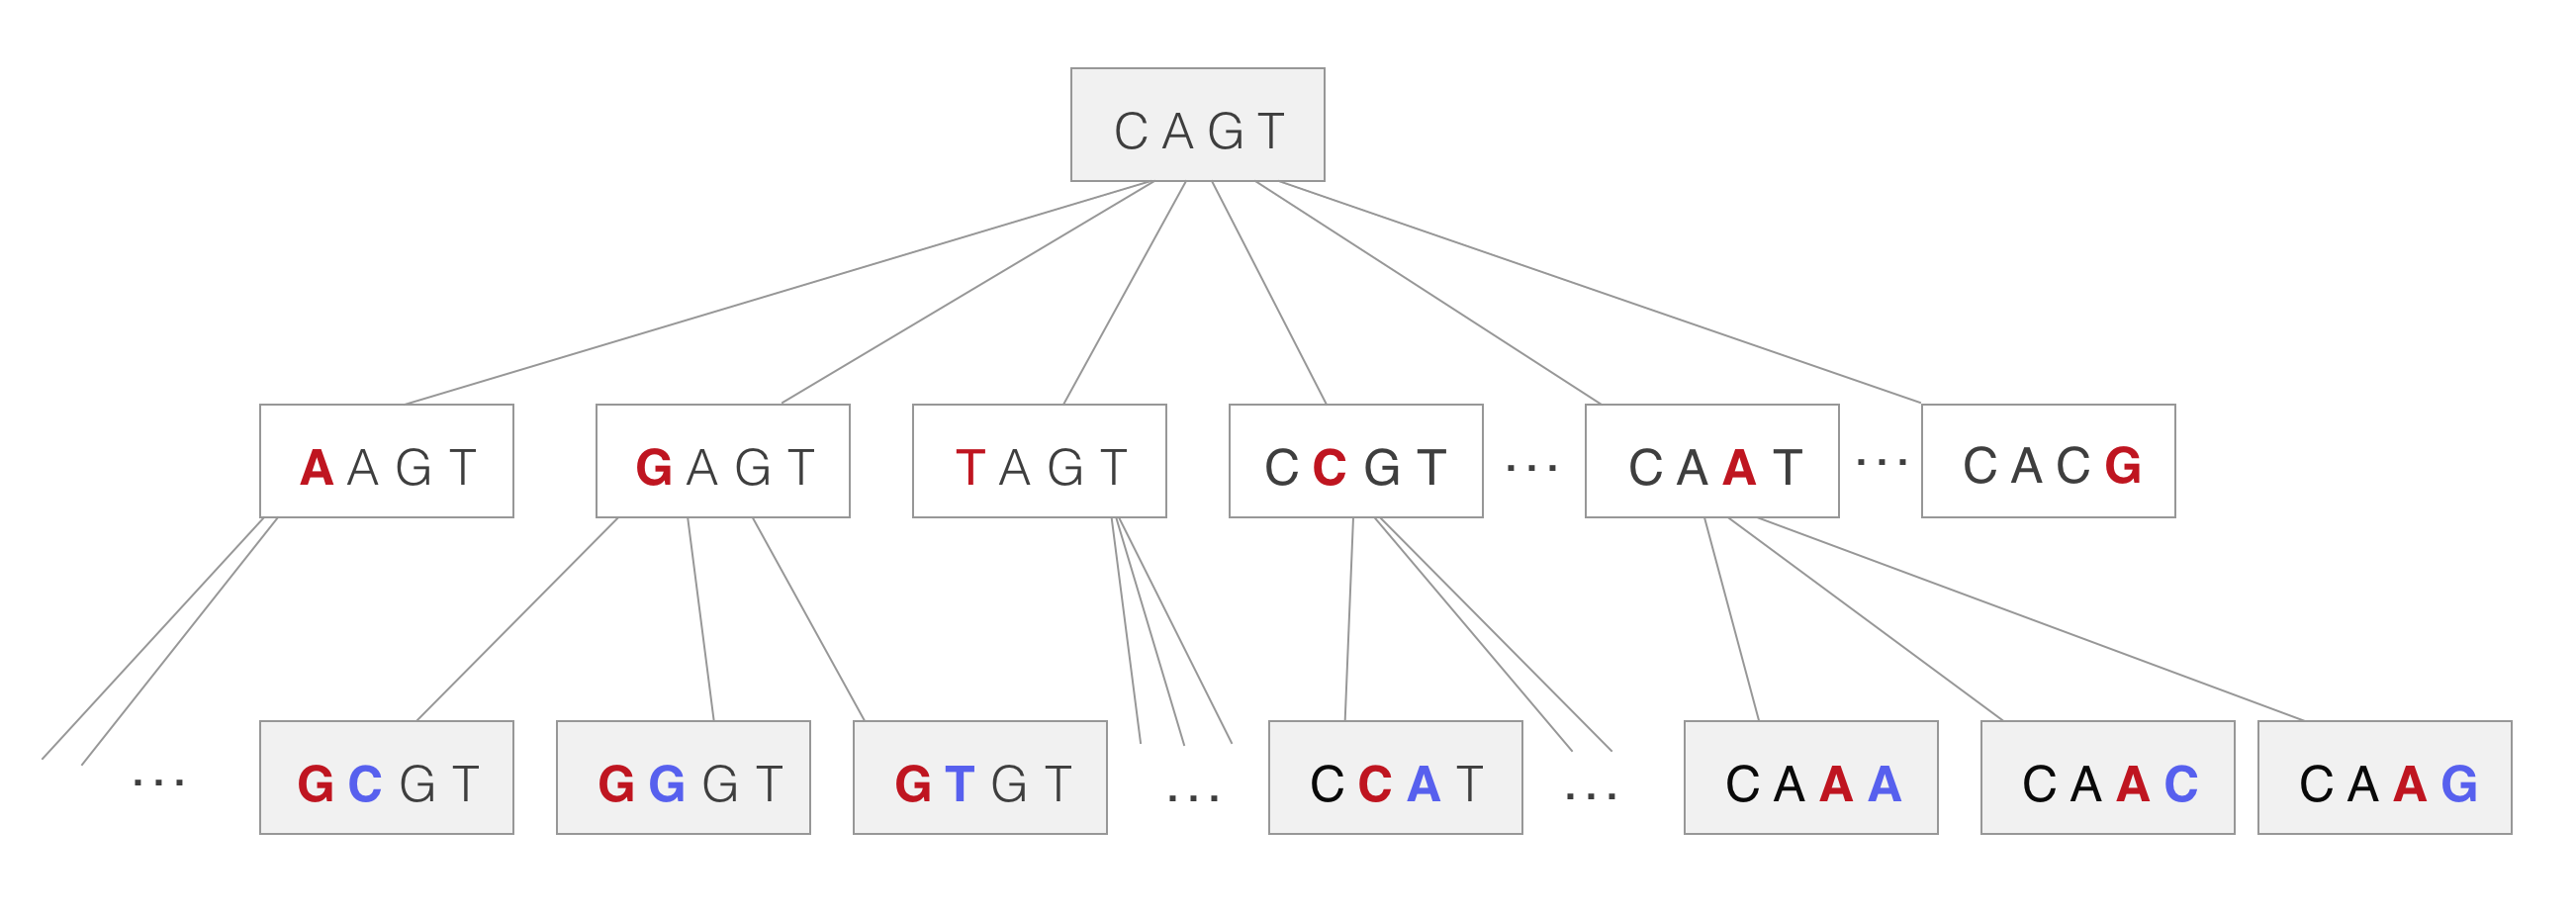
\includegraphics[width=5in]{contents/00_images/neighborhood-generation}\vspace*{5pt}
	\caption{Recursively generating the neighborhood of $l$-mer CACGT with $d = 2$}
	\label{fig:neighborhood-generation}
\end{figure}

	\subsubsection{Block-based optimization for neighborhood generation}
	The way EMS-GT represents the $d$-neighborhood $N_x$ of $l$-mer $x$ opens up a new way to improve the generation of neighborhood. $N_x$ is represented by a compresed $4^l$ bit flags array, where value of 1 corresponds to set membership, 0 if otherwise.  A previous study by Sia \cite{sia2015} improved the runtime performance in generating $N_x$. If $N_x$ is partitioned into blocks of $4^k$ bits each, where $k < l$, each block will conform into ($k$ + 2) bit patterns. By pre-computing these patterns, the algorithm can build the $N_x$ by blocks of bits instead of one bit at a time.

	\begin{figure}[h]
	\centering
	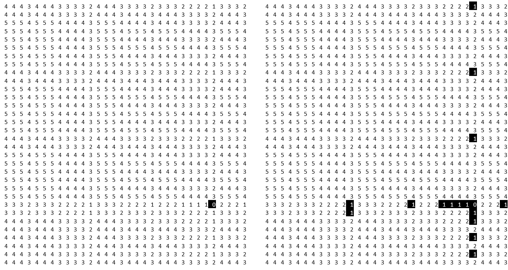
\includegraphics[width=2.5in]{contents/00_images/0-1}\vspace*{5pt}
	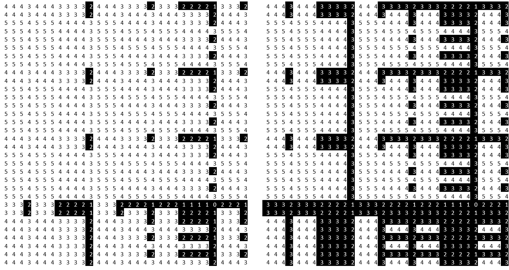
\includegraphics[width=2.5in]{contents/00_images/2-3}\vspace*{5pt}
	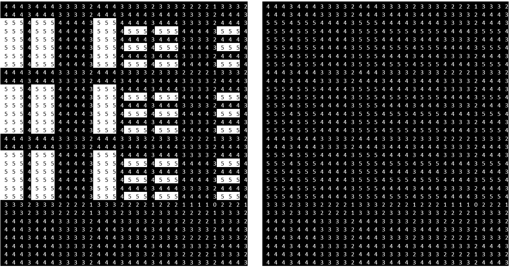
\includegraphics[width=2.5in]{contents/00_images/4-5}
	
	\caption{Bit patterns followed by blocks of size $4^{5}=32\times32$ in the bit-based representation of $\mathcal{N}(\texttt{acgtacgtacgt},5)$. Black signifies a 1. There are $(5+2)=7$ possible patterns---the empty pattern (all 0s) is not shown. Images from \cite{sia2015}}
	\label{fig:bit_patterns}
\end{figure}

	The algorithm divides the $l$-mer $x$ into its $(l - k)$-length prefix $y$ and suffix $z$ of length $k$. With the block patterns of $4^k$ $l$-mers generated, the algorithm recursively generates all possible prefix of $x$. For each prefix $y'$ generated, the algorithm applies the corresponding block pattern in $N_x$ based on $z$ and the remaining number of allowed mutations $d'$, where $d' = d - d_H(y, y')$. Specifically, EMS-GT builds the $\mathcal{N}_S$ using these steps:

	\begin{enumerate}
		\item Initialize $\mathcal{N}_S$ as an array of $4^l$ bits set to zero, and select a value for $k$.

		\item Pre-generate {\em Pattern}( $z$, $d_z$ ) for all $z \in \Sigma^k$ and all $d_z \in \{1,...,k-1\}$ to serve as bit masks for blocks. Note that block patterns for $d_z=0$ (one bit set) and $d_z=k$ (all bits set) will not require bit masks.

		\item For each $l$-mer $x = yz$ in sequence $S$: take each neighbor $y'$ of $y$, find the block in $\mathcal{N}_S$ whose prefix is $y'$, and compute the allowable suffix mismatches $d_z = d - d_H(y,y')$ within this block. Then,

			\begin{enumerate}
				\item if $d_z = 0$, set the bit at position $z$ in the block;
				\item if $d_z \geq k$, set all bits in the block to 1;
				\item otherwise, mask {\em Pattern}( $z$, $d_z$ ) onto the block.
			\end{enumerate}
	\end{enumerate}

	Choosing the optimum value for $k$ is important in this speedup technique. The $k$ value determines the runtime complexity of this technique since $k$ value determines the size of the block patterns. When $k$ value is higher, there are fewer prefix to generate recursively but each block bits setting is large. When $k$ value is lower, block bits setting is small but the algorithm has to recursively generate a larger number of prefix value of $l$-mer $x$. The optimum $k$ value used in the study is 5.

	
% {\setstretch{1.0} % Algorithm 4.1. Block Pattern Generation
\begin{figure}[h]
	\noindent \hspace*{6pt}{\bf Algorithm 2.1}
	\textsc{Block Pattern Generation}\small
	\begin{algorithmic}[1]\label{alg:block-pattern-gen}
		\Require block degree $k$
		\Ensure 3D bit-array $\mathcal{P}$ containing all possible non-trivial block patterns \vspace*{6pt}

		\State $\mathcal{P}[\ ][\ ][\ ] \leftarrow \{\}$ \hspace*{90pt}
		\Comment{retrieve a pattern $P$ as $\mathcal{P}[z][d - d_{y'}]$ }

		\For {$z \leftarrow 0$ to $4^k$}
		\For {$j \leftarrow 1$ to $k-1$}
		\For {$z' \leftarrow 0$ to $4^k$}
		\If{$dH(z,z') \leq j$} 
			\State $\mathcal{P}[z][j][z'] \leftarrow 1$
		\Else
			\State $\mathcal{P}[z][j][z'] \leftarrow 0$
		\EndIf\EndFor\EndFor\EndFor
		\State\Return $\mathcal{P}$
		\end{algorithmic}
\end{figure}



	% Elaborate and include results
	% Mention its competitiveness and a bit of introduction on possible areas of improvement 
	EMS-GT with this speedup technique has proven its competitiveness against algorithms qPMSPrune, qPMS7, PMS8 and qPMS9. Previous experimentations showed that EMS-GT with this speedup technique outperforms PMS8 in challenge instances (9, 2), (11, 3), (13, 4), (15, 5) and (17, 6). Compared to qPMS9, the improved EMS-GT is faster on all challenge instances mentioned except (17, 6). This study aims to outperform qPMS9 for challenges up to (17, 6).

	
\begin{figure}[ht]\label{fig:results2}
	\centering
	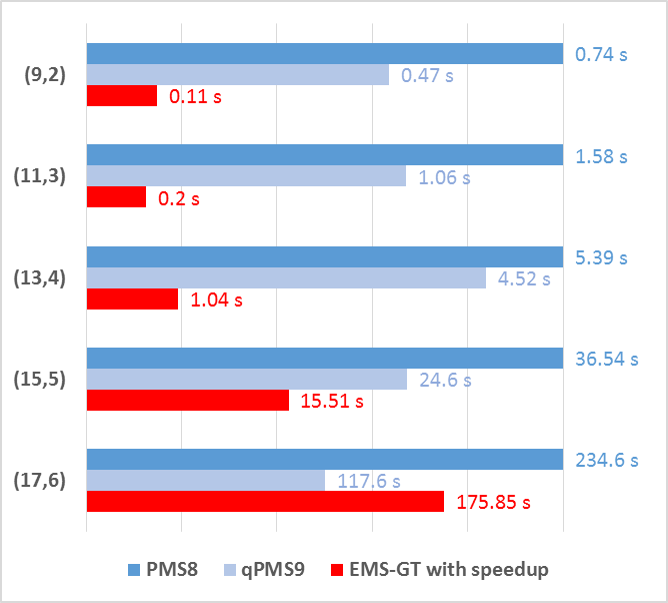
\includegraphics[width=4.0in]{contents/00_images/emsgt-with-speedup-vs-PMS,qPMS9}
	\caption{Improved EMS-GT's performance vs. PMS8 (baseline) and qPMS9. Images from \cite{sia2015}}
	\label{fig:sia-bar-results}
\end{figure}

% \begin{figure}[b]
	\noindent \hspace*{6pt}{\bf Algorithm 2} \textsc{Generate Neighborhood}
	\begin{algorithmic}[1]
		\label{alg:recursive-nbr-gen}
		\Require DNA sequence $S$, motif length $l$, mismatches $d$
		\Ensure bit-array $\mathcal{N}$ representing $\mathcal{N}(S,d)$ \vspace*{6pt}
		% \For{$i \leftarrow$ 1 to $4^{l}$}
		\State $\mathcal{N}[i] \leftarrow 0,\ \ \forall i < 4^{l}$ 
		% \EndFor
		\For{each $l$-mer $x$ in $S$}
			\State \textsc{AddNeighbors}($x$, 0, $d$) \hspace*{9pt}\Comment{recursive procedure}
		\EndFor
		\State \Comment{make $d$ changes in $l$-mer $x$, from position $s$ onward}
		\Procedure{AddNeighbors}{$x$, $s$, $d$}
			\For{$i \leftarrow s$ to $l$}
				\State $\Sigma \leftarrow$ \{\texttt{a}, \texttt{g}, \texttt{c}, \texttt{t}\} $- x_{i}$ \hspace*{6pt}\Comment{$i^{th}$ character in $x$}
				\For{$j \leftarrow 1$ to $|\Sigma|$}
					\State $neighbor \leftarrow\ ${\em\small concatenate}$(x_{1...i-1},\Sigma_{j},x_{i+1...l})$
					\State $\mathcal{N}[neighbor] \leftarrow 1$
					\If{$d > 1$ and $i < l$}
						\State \textsc{AddNeighbors}($neighbor$, $i+1$, $d-1$)
					\EndIf
				\EndFor
			\EndFor
		\EndProcedure
		\State\Return $\mathcal{N}$
	\end{algorithmic}
\end{figure}

Data structures and the how an algorithm deals with the data commonly drive the performance of an algorithm. The EMS-GT algorithm uses a compressed bit-flag array for fast candidate motif elimination. Some key techniques that EMS-GT uses are defined in this section.

	\subsubsection{Integer mapping of $l$-mers}
	EMS-GT converts $l$-mers into its corresponding integer values. To achieve this, each character in the $l$-mer is translated using 2 bits (a=00, c=01, g=10, t=11). \newline
		{\small Ex.	\texttt{actg} maps to \texttt{00011110} and has an integer value of 30} 

	\subsubsection{Bit-based set representation and l-mer enumeration} 
	The EMS-GT maintains a $4^l$ array for enumerating all the possible $l$-mer values. The $l$-mer's integer value is used as the index value for the array. It uses the value of 1 if the $l$-mer is a member of the set, else it sets the value to 0.

	\subsubsection{Bit-array compression}
	To efficiently store these $l$-mers and save memory space, EMS-GT implements an approach that compresses the search space array using integer value bit flags. Instead of one $l$-mer per index value, the implementation can flag up to 32 $l$-mers (since we are using 32-bit integers) per index value. The explanation on how the algorithm accesses the bit flag is defined below: \newline

		{\small Ex. \texttt{gacgt} maps to \texttt{1000011011} = 539 in decimal.\newline
			\hspace*{64pt} \emph{bit position} = 539 mod 32 = 27;\newline
			\hspace*{64pt} \emph{array index}  = 539 / 32 = 16;\newline
			\hspace*{64pt} The bit flag for \texttt{gacgt} is in the 27$^{th}$ least significant bit\newline
			\hspace*{64pt} of the integer at array index 16.}

	\begin{figure}[h]
	\centering
	\label{fig:search_space}
	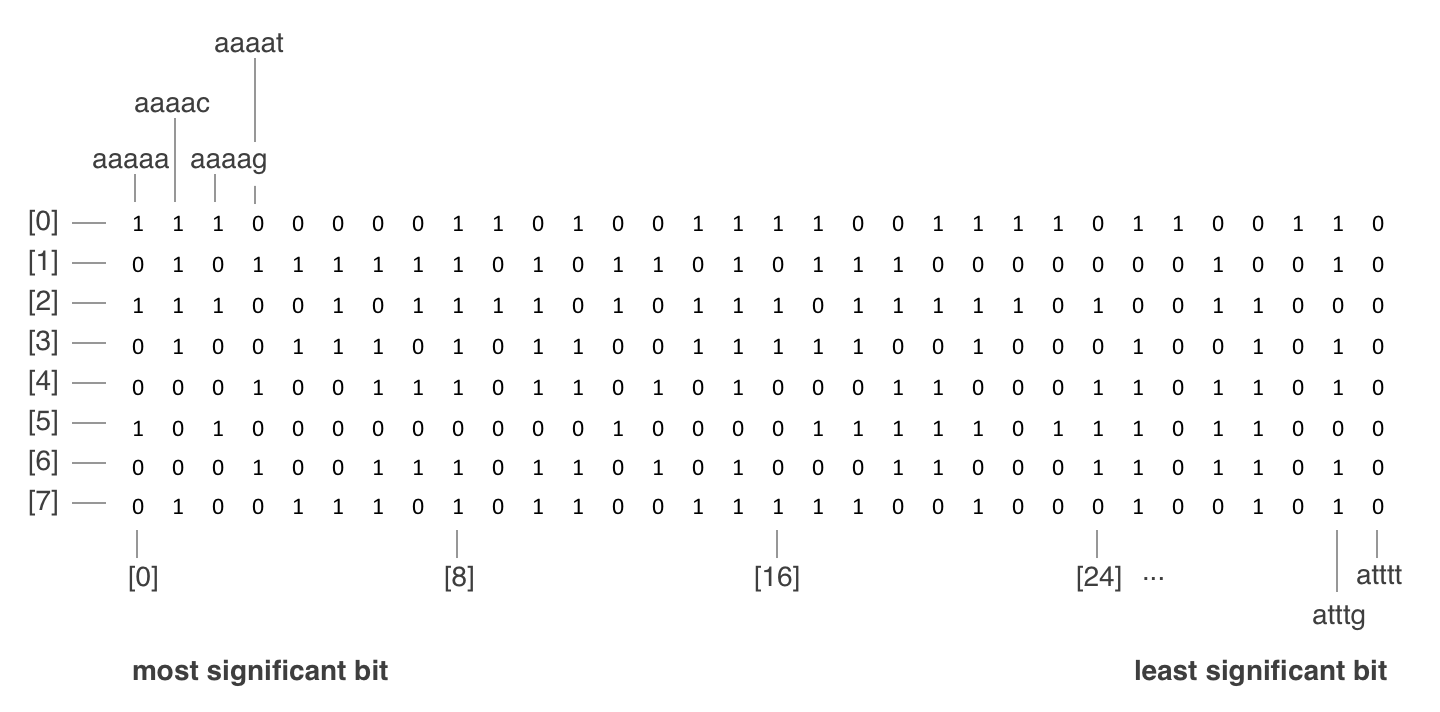
\includegraphics[width=5in]{contents/00_images/search_space}\vspace*{5pt}
	\caption{First 8 rows of the $4^{5}$ search space with random flag values.}
\end{figure}

	\subsubsection{XOR-based Hamming distance computation}
	The mapping of an $l$-mer to its integer value has an additional advantage in computing for mismatch positions. Applying the boolean operator exclusive-or (XOR) between two integer values will return another integer value that contains nonzero value for mismatch position. Counting this nonzero positions result to the hamming distance value. An example of this computation is shown below: \newline

	{\small Ex.	\texttt{aacgt} maps to \texttt{0000011011} \newline
		\vspace*{2pt}\hspace*{53pt} \underline{\texttt{tacgc} maps to \texttt{1100011001}} \newline
		\hspace*{55pt}	XOR produces \texttt{\uline{11}000000\uline{10}} = 2 mismatches.} \newline
		\hspace*{53pt} (Note, the mismatches are counted per pair)


	\subsubsection{Recursive neighborhood generation}
	The Generate step of the algorithm produces the $d$-neighborhood of a string sequence by generating the $d$-neighborhood of all $l$-mers in that sequence. Our implementation of EMS-GT uses a recursive approach for generating the $d$-neighborhood of an $l$-mer. The recursive generation can be visualized by a tree $\mathcal{T}(x)$ of height $d$ that is generated in depth-first manner. Each node is a tuple of $(w, p)$ where $w$ is an $l$-mer and $p$ corresponds to a position in the $l$-mer $0 \leq p \leq l$. At a given node $(w, p)$ and $p \neq l$, three children nodes are generated where each node is variant of $w$ that has a different character in $p + 1$ position. The root node is $(x, 0)$ and any $l$-mer in nodes at depth $t$ has a hamming distance of $t$ from the $l$-mer $x$. Given this, the expected size of $N(x, d)$ can be computed using the equation: \newline
	\begin{equation}
		|N(x,d)| = \sum_{i=0}^d \binom{l}{i} 3^{i}
	\end{equation}

	\begin{figure}[h]
	\centering
	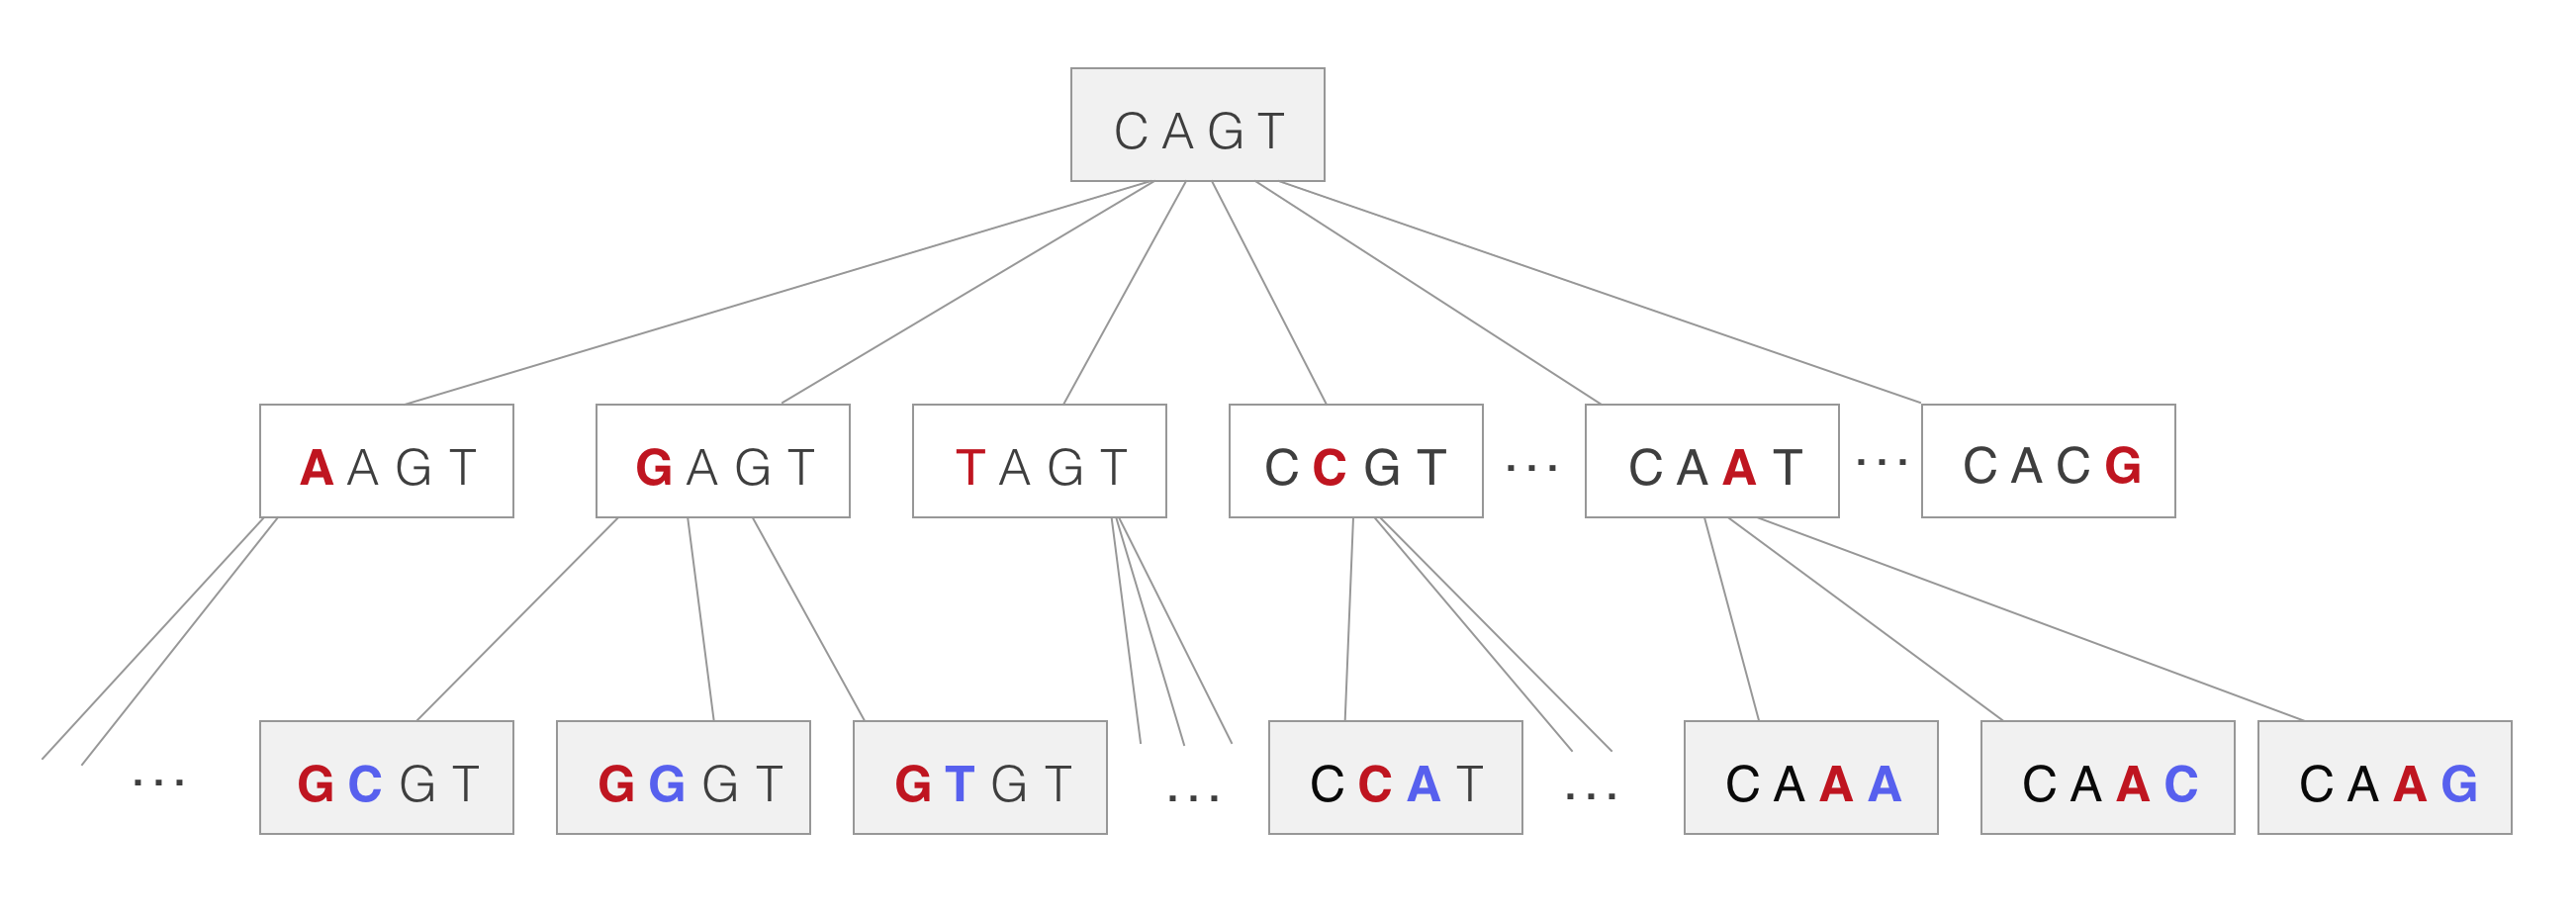
\includegraphics[width=5in]{contents/00_images/neighborhood-generation}\vspace*{5pt}
	\caption{Recursively generating the neighborhood of $l$-mer CACGT with $d = 2$}
	\label{fig:neighborhood-generation}
\end{figure}

	\subsubsection{Block-based optimization for neighborhood generation}
	The way EMS-GT represents the $d$-neighborhood $N_x$ of $l$-mer $x$ opens up a new way to improve the generation of neighborhood. $N_x$ is represented by a compresed $4^l$ bit flags array, where value of 1 corresponds to set membership, 0 if otherwise.  A previous study by Sia \cite{sia2015} improved the runtime performance in generating $N_x$. If $N_x$ is partitioned into blocks of $4^k$ bits each, where $k < l$, each block will conform into ($k$ + 2) bit patterns. By pre-computing these patterns, the algorithm can build the $N_x$ by blocks of bits instead of one bit at a time.

	\begin{figure}[h]
	\centering
	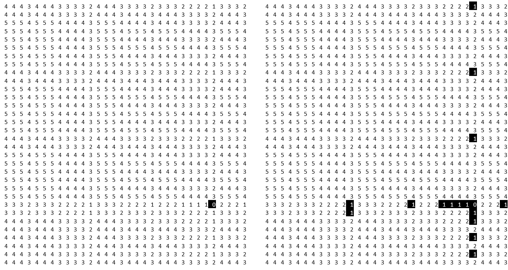
\includegraphics[width=2.5in]{contents/00_images/0-1}\vspace*{5pt}
	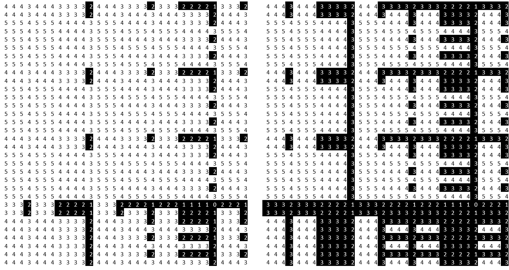
\includegraphics[width=2.5in]{contents/00_images/2-3}\vspace*{5pt}
	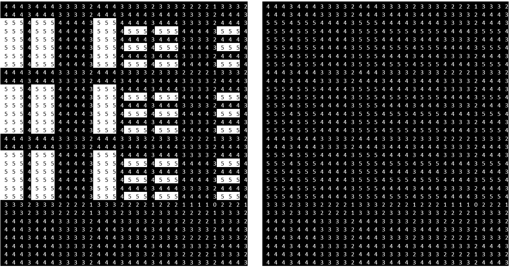
\includegraphics[width=2.5in]{contents/00_images/4-5}
	
	\caption{Bit patterns followed by blocks of size $4^{5}=32\times32$ in the bit-based representation of $\mathcal{N}(\texttt{acgtacgtacgt},5)$. Black signifies a 1. There are $(5+2)=7$ possible patterns---the empty pattern (all 0s) is not shown. Images from \cite{sia2015}}
	\label{fig:bit_patterns}
\end{figure}

	The algorithm divides the $l$-mer $x$ into its $(l - k)$-length prefix $y$ and suffix $z$ of length $k$. With the block patterns of $4^k$ $l$-mers generated, the algorithm recursively generates all possible prefix of $x$. For each prefix $y'$ generated, the algorithm applies the corresponding block pattern in $N_x$ based on $z$ and the remaining number of allowed mutations $d'$, where $d' = d - d_H(y, y')$. Specifically, EMS-GT builds the $\mathcal{N}_S$ using these steps:

	\begin{enumerate}
		\item Initialize $\mathcal{N}_S$ as an array of $4^l$ bits set to zero, and select a value for $k$.

		\item Pre-generate {\em Pattern}( $z$, $d_z$ ) for all $z \in \Sigma^k$ and all $d_z \in \{1,...,k-1\}$ to serve as bit masks for blocks. Note that block patterns for $d_z=0$ (one bit set) and $d_z=k$ (all bits set) will not require bit masks.

		\item For each $l$-mer $x = yz$ in sequence $S$: take each neighbor $y'$ of $y$, find the block in $\mathcal{N}_S$ whose prefix is $y'$, and compute the allowable suffix mismatches $d_z = d - d_H(y,y')$ within this block. Then,

			\begin{enumerate}
				\item if $d_z = 0$, set the bit at position $z$ in the block;
				\item if $d_z \geq k$, set all bits in the block to 1;
				\item otherwise, mask {\em Pattern}( $z$, $d_z$ ) onto the block.
			\end{enumerate}
	\end{enumerate}

	Choosing the optimum value for $k$ is important in this speedup technique. The $k$ value determines the runtime complexity of this technique since $k$ value determines the size of the block patterns. When $k$ value is higher, there are fewer prefix to generate recursively but each block bits setting is large. When $k$ value is lower, block bits setting is small but the algorithm has to recursively generate a larger number of prefix value of $l$-mer $x$. The optimum $k$ value used in the study is 5.

	
% {\setstretch{1.0} % Algorithm 4.1. Block Pattern Generation
\begin{figure}[h]
	\noindent \hspace*{6pt}{\bf Algorithm 2.1}
	\textsc{Block Pattern Generation}\small
	\begin{algorithmic}[1]\label{alg:block-pattern-gen}
		\Require block degree $k$
		\Ensure 3D bit-array $\mathcal{P}$ containing all possible non-trivial block patterns \vspace*{6pt}

		\State $\mathcal{P}[\ ][\ ][\ ] \leftarrow \{\}$ \hspace*{90pt}
		\Comment{retrieve a pattern $P$ as $\mathcal{P}[z][d - d_{y'}]$ }

		\For {$z \leftarrow 0$ to $4^k$}
		\For {$j \leftarrow 1$ to $k-1$}
		\For {$z' \leftarrow 0$ to $4^k$}
		\If{$dH(z,z') \leq j$} 
			\State $\mathcal{P}[z][j][z'] \leftarrow 1$
		\Else
			\State $\mathcal{P}[z][j][z'] \leftarrow 0$
		\EndIf\EndFor\EndFor\EndFor
		\State\Return $\mathcal{P}$
		\end{algorithmic}
\end{figure}



	% Elaborate and include results
	% Mention its competitiveness and a bit of introduction on possible areas of improvement 
	EMS-GT with this speedup technique has proven its competitiveness against algorithms qPMSPrune, qPMS7, PMS8 and qPMS9. Previous experimentations showed that EMS-GT with this speedup technique outperforms PMS8 in challenge instances (9, 2), (11, 3), (13, 4), (15, 5) and (17, 6). Compared to qPMS9, the improved EMS-GT is faster on all challenge instances mentioned except (17, 6). This study aims to outperform qPMS9 for challenges up to (17, 6).

	
\begin{figure}[ht]\label{fig:results2}
	\centering
	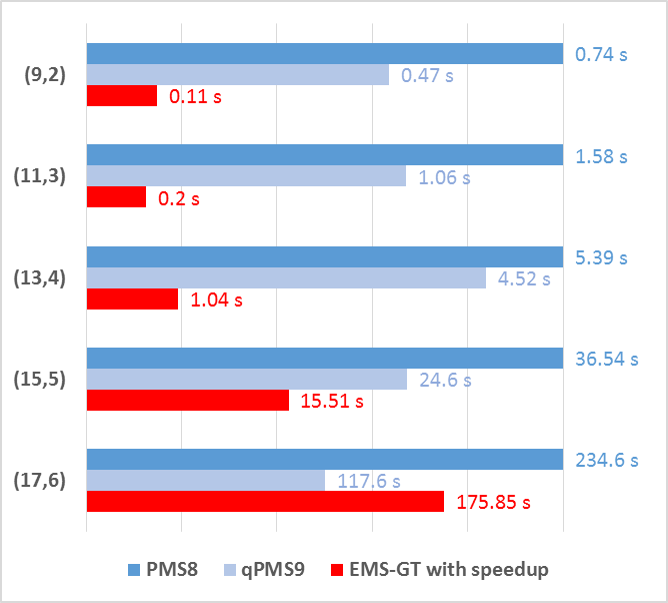
\includegraphics[width=4.0in]{contents/00_images/emsgt-with-speedup-vs-PMS,qPMS9}
	\caption{Improved EMS-GT's performance vs. PMS8 (baseline) and qPMS9. Images from \cite{sia2015}}
	\label{fig:sia-bar-results}
\end{figure}

		% CHAPTER 3
		\chapter{METHODOLOGY}
			This section describes how the speedup-techniques was explored and implemented. Each algorithm was evaluated using the $(9, 2)$, $(11, 3)$, $(13, 4)$, $(15, 5)$ and $(17, 6)$ challenge instances. An $(l, d)$ problem instance is said to be challenging if $d$ is the largest integer value for which the expected number of motifs of lenght $L$ would occur in the input by random chance and does not exceed a constant value (500) \cite{pms2015}.

\begin{figure}[h]
	\centering
	\label{fig:methodology}
	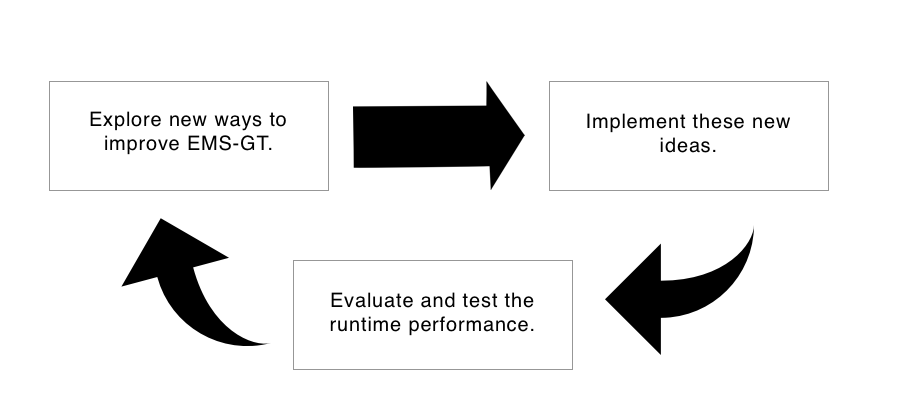
\includegraphics[width=5.5in]{contents/00_images/methodology}
	\caption{Speedup Technique Development Cycle.}
\end{figure} 

The study aims to improve the algorithm by pre-computation of values and exploring other usage of the block-processing technique. The speedup techniques were developed using the development cycle shown in Figure \ref{fig:methodology}.

\section{Improving the EMS-GT}
%  C++ implementation
Originally, EMS-GT was implemented using Java, but for the purpose of eliminating variables that may affect the evaluation of the algorithms, it was converted to C++. 

% block flags
A previous study \cite{sia2015} improved the neighborhood generation by setting the neighborhood array by blocks of bits instead of one bit at a time. The Generation phase quickly filters the candidate motifs array as it processes the first $n'$ sequences, leaving numerous empty blocks of $l$-mers in the candidate motifs array. It was observed that at some point in the Generation phase, some of the block settings are not necessary anymore since that block is already empty in the candidate motifs array. We improved the algorithm by maintaining boolean flags for those empty blocks and then we ignore all block bit settings for those blocks. Additionally, the block-processing procedure was found useful in testing of candidate motifs. The Test phase checks if a candidate motif $c$ is in the remaining $n - n'$ sequences by comparing if there is at least one $l$-mer in each sequence that is within $d$-distance from $c$. If a candidate motif $x$ is eliminated for failing to have a $d$-neighbor in some input sequence $S_i$, that it is possible to reduce the testing for another candidate motif $y$ on the same sequence $S_i$, if y is within the same $k$-block as x.

% pre computation
Hamming distance computation was also improved using a pre-computed lookup values. Given an XOR result, instead of counting nonzero pairs of bits, we use the lookup table to get the number of mismatches. Lastly, we explored a pruning strategy in generation of neighborhood of a sequence.

% n' values then parameter fine tuning

\section{Parameter Fine Tuning}
The EMS-GT algorithm defines an integer value $n'$ ($1 < n' < n$) that divides the dataset into two smaller set of sequences. The first n' sequences are used in the Generate phase while the remaining is assigned to the Test phase. Previous experimentations \cite{sia2015} showed that it is efficient for the algorithm to set the value of $n'$ to 10. Technically, $n'$ dictates hwo big is the size of the set of candidate motifs \mathcal{C} to be evaluated if they are in the remaining $n - n'$ sequences. In line with this, we run an experimentation that records the average runtime of the algorith mwith the speedup techniques over 5 tests and having different values for $n'$. The values for $n'$ range from 5 to 10 in this experiment, since we only want to make the candidate motifs set large enough for our speedup technique to take effect.

\section{Evaluation}


\subsection{Datasets}




		% CHAPTER 4
		\chapter{RESULTS AND DISCUSSION}
			\section{Results}

This section describes speedup techniques that is incorporated with EMS-GT and briefly discusses the observation where the idea for the improvement originated. 

\section{Pruning strategy in Neighborhood Generation of a Sequence}
% rephrase
EMS-GT generates the $d$-neighborhood of a sequence by collecting all the $d$-neighbors of every $l$-mer in the sequence. 

% rephrase
It is obvious that identical $l$-mers has a hamming distance of 0 and will generate the same $d$-neighborhood. Thus we only need to generate the $d$-neighborhood of distinct $l$-mers in a sequence. This observation can be extended into a pruning strategy as we process the neighborhood generation of $l$-mers in a sequence.

% DEFER
\section{Block flags implementation in Generate phase}

The EMS-GT algorithm follows the pattern-driven approach where it exhaustively tests the $4^l$ bit-array of possible motifs. It quickly filters the $4^l$ bit-array in the Generate phase by intersecting the $d$-neighborhood of the first $n'$ sequences. To be specific, EMS-GT maintains two $4^l$ bit-array during the Generate phase. The first array holds the remaining candidate motifs and the second array holds the $d$-neighborhood of the current sequence. For every sequence in the first $n'$ sequences, we generate the $d$-neighborhood by blocks then interects it with the candidate motifs array, the resulting set will be the new candidate motifs array. We observed that at some point in the Generation phase, candidate motifs array has numerous empty blocks of $l$-mers. Applying block masks in this part of the neighbordhood array will be useless since we already know that there is no candidate motifs in that block. An efficient way is to focus the neighborhood generation on those blocks where there are still candidate motifs. We have implemented a block flags strategy that tracks these empty blocks in the candidate motifs array.

% Figure that shows empty blocks in candidate motifs array

\subsection{Faster Candidate Motif Elimination through Block Processing}

The EMS-GT algorithm tests candidate motifs in a brute-force approach. A candidate motif is tested by checking if each of the remaining $(n - n')$ sequences contains an $l$-mer that has at most $d$ hamming distance value with the candidate motif. In testing a candidate motif $c$, if there is a sequence $S_i$ in $(n - n')$ that has no $l$-mer with hamming distance of at most $d$ with $c$, the candidate motif $c$ is automatically eliminated.

Since the search space is represented by a compressed bit array and the $l$-mers are enumerated alphabetically, $l$-mers that are near each other share the same $p$-length prefix string. We used this observation in improving the way the algorithm tests the candidate motifs. In EMS-GT, each testing of candidate motif is independent of each other. We proposed a speedup technique that processes these candidate motifs by block. Dividing the search space and grouping the $l$-mers by fix block $k$ will result into a group of $l$-mers that has the same $(l - k)$-length prefix where $k < l$. We can easily observe that increasing the value of $k$-block size will increase the number of $l$-mers in a group but decreases the length of the common prefix string they share. If candidate motifs $x$ and $y$ are within $k$-block and $x$ has been eliminated as a candidate motif in sequence $S_i$ $(n' \leq i \leq n)$, we can filter out $l$-mers $z \in S_i$ where $d_H(x,z) > d + k$. We collect the remaining $l$-mers in $S_i$ and use it for testing the remaining candidate motifs in the block along with the other $l$-mers in the remaining sequences. 

\begin{thm} \label{thm:triangle}
	Let x and y be $l$-mers in a $k$-size block in the search space and $d_H(x, y) \leq k$. Let $d$ be the number of allowed mutations in the problem. Let z be another $l$-mer. If $d_H(x, z) > (d + k)$ then $d_H(y, z) > d$ and $z \not\in N(y, d)$
\end{thm}

\begin{proof}[Proof of Theorem \ref{thm:triangle}]
Using proof by contradiction, suppose that $d_H(y, z) \leq d$. We know that $d_H(x, z) < d_H(y, z) + d_H(x, y)$ from the triangle inequality. We can write this equation into $d_H(x, z) < d + k$ thus a contradiction to the previous assumption that $d_H(x, z) > (d + k)$.
\end{proof}


\subsection{Pre-computation of Mismatch Values}
The EMS-GT2 uses the hamming distance computation heavily on the Test phase. To compute the hamming distance of two binary represented $l$-mers, the algorithm uses the boolean operator XOR between the two $l$-mers and results an integer with nonzero pair of bits at every mismatch position. Counting these pair of bits will result to the hamming distance value. The total number of pairs of bits is equal to the length of the motif and is also equal to the total number of comparisons it has to do in the hamming distance computation. 

Instead of repeatedly counting this nonzero pairs of bits everytime we compute the hamming distance, using a lookup table of nonzero pair of bits count for all possible integer values will help save computational time. Although, pre-computing these nonzero pair counts for all possible 32 bit values will introduce an overhead computation problem. A more efficient approach is to pre-compute only up to $b$ number of bits where $b < 32$ and $b$ is an even number. Then we count for the hamming distance by looking up the nonzero counts $b$ number of bits at a time as shown in \ref{alg:upd-hamming-distance-comp}. In our implementation, we pre-compute up to 18 bit values only.

\begin{figure}[h]
	\noindent \hspace*{6pt}{\bf Algorithm 4} \textsc{Hamming Distance Computation using Pre-Computed Mismatch Values}
	\begin{algorithmic}[1]
		\label{alg:upd-hamming-distance-comp}
		\Require $l$-mer mappings $u$ and $v$ and\newline
			\hspace*{8pt} MC \Comment{array of pre-computed count of mismatch positions}
		\Ensure Hamming distance $d_H(u,v)$ \vspace*{6pt}
		\State $d_H(u, v) \leftarrow 0$
		\State $z \leftarrow u \oplus v$
		\While{$z > 0$}
			\State $l \leftarrow z \& ((1 << 18) - 1)$
			\State $d_H(u, v) \leftarrow d_H(u, v) + MC[l]$ 
			\State $z \leftarrow z >>> 18$ \Comment{shift 18 bits to the right}
		\EndWhile
		\State\Return $d_H(u, v)$
	\end{algorithmic}
\end{figure} 










% Runtime results
\section{Performance of EMS-GT with speedup techniques}

% Pruning -- 

% Block Flags only

% Faster Candidate Motif only

% Block Flags + HD

% Faster Candidate Motif + HD

% Block Flags + Faster Candidate Motif + HD


The EMS-GT2, EMS-GT and qPMS9 was evaluated using Intel Xeon, 2.10 Ghz machine. The performance of each algorithm was averaged over 20 synthetic datasets for each $(l, d)$-challenge instance where $l \leq 17$. Table \ref{tbl:final-results-ems} shows the runtime results between EMS-GT2 vs EMS-GT while table \ref{tbl:final-results} shows the runtime results between EMS-GT2 vs the state-of-the-art algorithm qPMS9.

\begin{table}[h] %speedup_blockmasking
	\renewcommand{\arraystretch}{1.3}
	\centering
	\begin{tabular}{|c|c|c|c|}
	\hline 
	\bfseries\boldmath $(l,d)$ & 
	\bfseries EMS-GT & 
	\bfseries\boldmath EMS-GT2  & 
	\bfseries \% speedup\\
	\hline
	 (9,2) 	&  0.047 s &    0.038 s &    18.33 \%\\
	(11,3) &   0.168 s &    0.126 s &    25.46 \%\\
	(13,4) &   1.181 s &    0.946 s &   19.88 \%\\
	(15,5) &  12.768 s &   10.876 s &   14.81 \%\\
	(17,6) & 143.215 s &  111.660 s &   22.03 \%\\
	\hline\end{tabular}
	
	\caption{EMS-GT and EMS-GT2 runtime evaluation.}
	\label{tbl:final-results-ems}
\end{table}

% Explanation for Table final-results-ems
The additional speedup techniques become more efficient as the $l$ value in the $(l, d)$-instance grows. For every $(l, d)$-challenge instances mentioned where $l \geq 13$, EMS-GT2 has improved the runtime over the EMS-GT for at least 15\%. Unfortunately, the speedup techniques in EMS-GT2 failed to compensate for their additional overhead computations in both $(9, 2)$ and $(11, 3)$ challenge instances and failed to improve the overall runtime of the implementation.

\begin{table}[h] %speedup_blockmasking
	\renewcommand{\arraystretch}{1.3}
	\centering
	\begin{tabular}{|c|c|c|c|}
	\hline 
	\bfseries\boldmath $(l,d)$ & 
	\bfseries qPMS9 & 
	\bfseries\boldmath EMS-GT2 & 
	\bfseries \% speedup\\
	\hline
	 (9,2) &   0.647 s &    0.039 s &   93.97 \%\\
	(11,3) &   1.276 s &    0.140 s &   89.02 \%\\
	(13,4) &   4.269 s &    0.758 s &   82.24 \%\\
	(15,5) &  24.737 s &   10.565 s &   57.29 \%\\
	(17,6) & 118.226 s &  112.311 s &   5.00 \%\\
	\hline\end{tabular}
	
	\caption{EMS-GT2 and qPMS9 runtime evaluation.}
	\label{tbl:final-results}
\end{table}



% Explanation for Table final-results
Previous implementations of EMS-GT2 failed to beat qPMS9 in $(17, 6)$-challenge instance. EMS-GT2 not only improved the runtime of the implementation but also succeed in beating the qPMS9 in this challenge instance. The implementation of EMS-GT now is faster than the state-of-the-art qPMS9 in all of the $(l, d)$-challenge instances where $l \leq 17$. Even though the implementation of EMS-GT can only run in $(l, d)$-challenge instances where $l \leq 17$ because of memory constraint, studies shown that the typical length of motifs is around 10 base pairs (bp) \cite{stewart2012transcription}










		% CHAPTER 5
		\chapter{CONCLUSION}
			\section{Conclusions}

We have presented EMS-GT2, an improved exact solution for the planted-motif search problem. EMS-GT2 was able to efficiently test candidate motifs in block by filtering out $l$-mers using a property of the search space array that we have discovered. The previous implementation of EMS-GT already outperforms the state-of-the-art algorithm qPMS9 in $(l, d)$-challenge instances $(9, 2)$, $(11, 3)$, $(13, 4)$ and $(15, 5)$ but failed to beat qPMS9 in $(17, 6)$-challenge instance. EMS-GT2 improved the algorithm's performance on $(13, 4)$, $(15, 5)$ and $(17, 6)$ and was able to beat qPMS9 in all $(l, d)$-challenge instances where $l \leq 17$.

	% \BackMatter
		\bibliographystyle{plain}
		\bibliography{sources}

	\addappheadtotoc
	\begin{appendices}
		\appendix{Source Code Repository of the EMS-GT2 algorithm}

\begin{footnotesize}

The source codes and codes used for experimentations are stored in github repository. The link for the repository is https://github.com/markronquillo/thesis.

\end{footnotesize}
		\appendix{ECBA 2016 Conference Paper}
	\label{appendix:MNE-586-105}
	\centering{\textbf{Accepted and Presented}}
	
	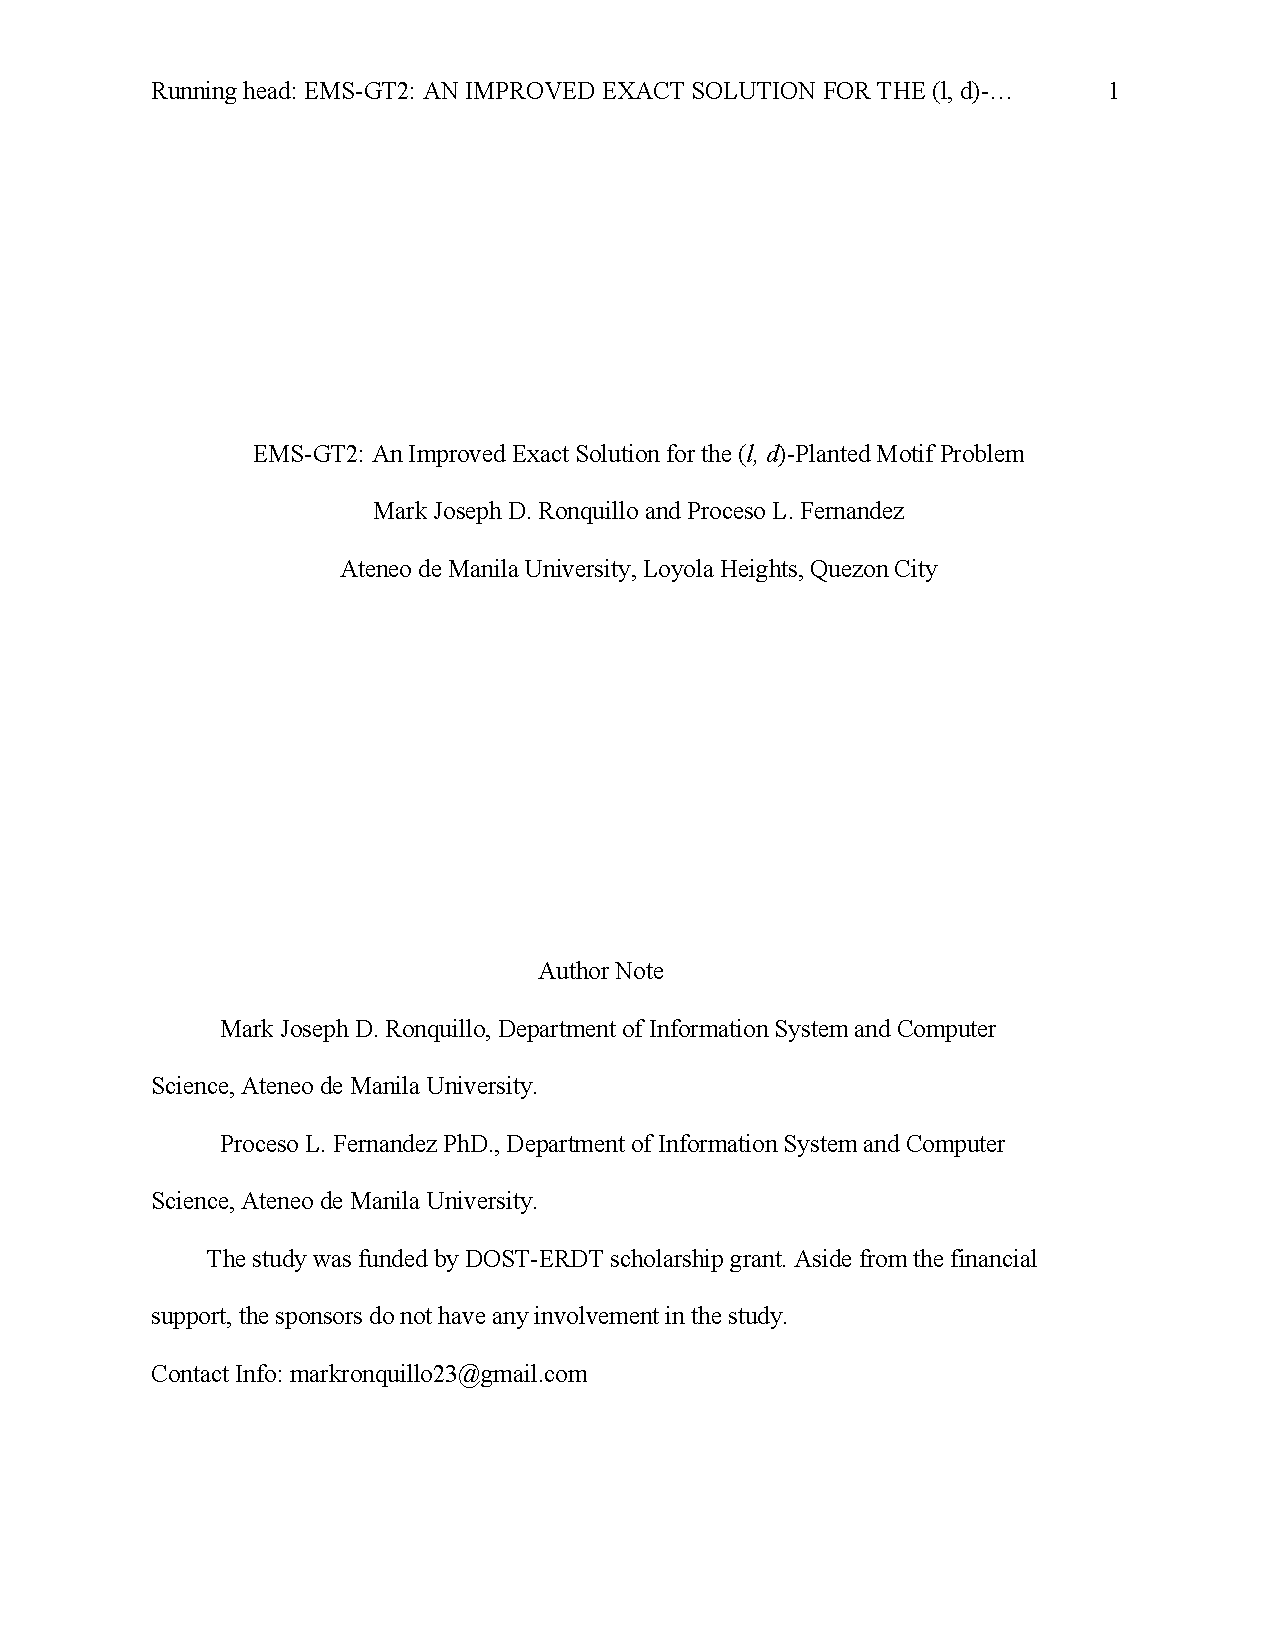
\includegraphics[page=1, scale = 0.8]{contents/appendix/MNE-586-105.pdf}
	\includegraphics[page=2, scale = 0.8]{contents/appendix/MNE-586-105.pdf}
	\includegraphics[page=3, scale = 0.8]{contents/appendix/MNE-586-105.pdf}
	\includegraphics[page=4, scale = 0.8]{contents/appendix/MNE-586-105.pdf}
	\includegraphics[page=5, scale = 0.8]{contents/appendix/MNE-586-105.pdf}
	\includegraphics[page=6, scale = 0.8]{contents/appendix/MNE-586-105.pdf}
	\includegraphics[page=7, scale = 0.8]{contents/appendix/MNE-586-105.pdf}
	\includegraphics[page=8, scale = 0.8]{contents/appendix/MNE-586-105.pdf}
	\includegraphics[page=9, scale = 0.8]{contents/appendix/MNE-586-105.pdf}
	\includegraphics[page=10, scale = 0.8]{contents/appendix/MNE-586-105.pdf}
	\includegraphics[page=11, scale = 0.8]{contents/appendix/MNE-586-105.pdf}
	\includegraphics[page=12, scale = 0.8]{contents/appendix/MNE-586-105.pdf}
	\includegraphics[page=13, scale = 0.8]{contents/appendix/MNE-586-105.pdf}
	\includegraphics[page=14, scale = 0.8]{contents/appendix/MNE-586-105.pdf}
	\includegraphics[page=15, scale = 0.8]{contents/appendix/MNE-586-105.pdf}
	\includegraphics[page=16, scale = 0.8]{contents/appendix/MNE-586-105.pdf}
	\includegraphics[page=17, scale = 0.8]{contents/appendix/MNE-586-105.pdf}
	\includegraphics[page=18, scale = 0.8]{contents/appendix/MNE-586-105.pdf}
	\includegraphics[page=19, scale = 0.8]{contents/appendix/MNE-586-105.pdf}
	\includegraphics[page=20, scale = 0.8]{contents/appendix/MNE-586-105.pdf}
	\includegraphics[page=21, scale = 0.8]{contents/appendix/MNE-586-105.pdf}
	\includegraphics[page=22, scale = 0.8]{contents/appendix/MNE-586-105.pdf}
	\includegraphics[page=23, scale = 0.8]{contents/appendix/MNE-586-105.pdf}
	\includegraphics[page=24, scale = 0.8]{contents/appendix/MNE-586-105.pdf}



	\end{appendices}

  
\end{document}
